\chapter{Choosing among protection settings}\label{ch:selection}

Chapter~\ref{ch:estimate} gave a committee a rule for one setting: release only if the
exact upper bound on the declared risk is at or below the tolerance. In practice a
committee rarely faces one setting. It faces a menu: minimum cell counts of 1, 5, 10 and
upwards, coarser and finer classifications, more or less suppression. The procedure that
most analysts follow next seems to need no defence. Test every setting on the menu with
the bound rule, set aside those that fail, and among those that pass choose the one that
costs the users least.

The procedure deserves its strongest statement. Each setting is tested with a valid
bound at level $\alpha$, so each setting that passes has passed an honest test. Choosing
among the passing settings is an ordinary constrained optimisation: maximise the value of
the release subject to the risk constraint, which is how the risk--utility literature
frames mechanism choice \citep{duncan2001}. An analyst who chose a more protective
setting than the least protective one that passes would throw away utility and gain
nothing that the test had not already secured. On this view the menu is a convenience,
and the guarantee of Chapter~\ref{ch:estimate} carries over to whichever setting is
chosen.

The guarantee does not carry over, and simple arithmetic shows why. The setting that is
chosen was chosen with the same bounds that certify it. Suppose five settings on the menu
are unsafe, each with a true risk just above the tolerance, and each is tested on its own
independent draw of targets at $\alpha = 0.05$. Each passes falsely with probability up
to 0.05, and the procedure picks the least protective setting that passes, which will be
an unsafe one whenever any unsafe setting passes. The chance that at least one of five
passes is $1 - 0.95^5 = 0.226$, four and a half times the level the committee believes
it is working at.
% arithmetic: 1 - 0.95^5 = 0.2262 (a calculation from Proposition c05:prop-scan, not a repository output)
With more unsafe settings near the line it grows further. Each test was honest; the
choice among them was not tested at all.

\begin{example}[How the error grows with the menu]\label{c05:ex-menu}
Take Naledi's menu of thirteen floors and suppose that some of them are unsafe, each with
a true risk so close to the tolerance that its bound passes with probability 0.05, and
that each floor is tested on its own draw of targets. With two unsafe floors the scan
picks an unsafe one with probability $1 - 0.95^2 = 0.098$. With five it is
$1 - 0.95^5 = 0.226$, and with ten it is $1 - 0.95^{10} = 0.401$. In the last case a
committee that believes it works at 5 per cent releases an unsafe floor two times in
five, and since it cannot know in advance how many floors sit near the line, it cannot
know which of the three figures applies to it.
\end{example}

Clinical trials met this problem decades ago. A sponsor testing several doses of a drug
against a placebo, and claiming an effect for whichever doses beat it, multiplies its
chances of a false claim. \citet{maurer1995} described the remedy for the case in which
the hypotheses can be put in order before the data are seen, as doses can: test them in
that order, each at the full level, and stop at the first that fails. A disclosure grid
has the same structure, because its settings can be ordered by how much protection they
give before any attack is simulated.

The chapter therefore asks one question. How can a committee choose a protection setting
from a menu, using the same simulated evidence that certifies it, and keep the chance of
releasing an unsafe setting at its stated level?

\section{A request for loan-level data}

At the Bank the question arose from a request by Tomás, a visiting researcher, for a
loan-level extract of the credit register: one record per loan, with the borrower's
sector, region and size class and the amount of the exposure, released monthly. The
evidence in this chapter comes from the synthetic register that stands in for the Bank's,
with 20,000 borrowing firms, 60 lenders and six monthly vintages, of which the first
holds 27,167 loans.
% source: paper/generated/numbers.tex (\runcreditborrowers, \runcreditlenders, \runevalperreleasekept); paper/bis_ifc_full.tex line 2201 ff.
Its parameters were chosen, not estimated from a real register, and the floors reported
below inherit those choices: exposures that do not change over time and lending activity
that does not depend on firm size are two of them.

Naledi's protection lever was a minimum cell count on the key of sector, region and size
class, with loans in smaller cells suppressed. Her menu held thirteen floors, from 1,
meaning no suppression, through 5, 10, 15, 20, 30, 40, 50, 75, 100, 150 and 200 to 300.
% source: scripts/programme_robustness.py (LEVELS)
The committee's tolerance was 0.12 at an error level of 0.05.
% source: scripts/programme_robustness.py (TOLERANCE, ALPHA); paper/generated/table_robustness.tex
Tomás asked, reasonably, for the lowest floor that passed. A lower floor kept more loans,
and the loans that a higher floor removed were the large ones, in the thin cells, which
were the ones his research was about.

\section{The constrained choice}

Write $\Theta$ for the menu of settings, $U(\theta)$ for the utility of the release under
setting $\theta$, declared in advance as a loss on the analyses the users will run, and
$\overline{R}_{1-\alpha}(t,\theta)$ for the exact bound for target set $T$. The choice
the committee wants to make is
\begin{equation}\label{c05:eq-opt}
\theta^\star \in \arg\max_{\theta \in \Theta} U(\theta)
\quad \text{subject to} \quad
\sup_{t \in T}\overline{R}_{1-\alpha}(t,\theta) \le \tau .
\end{equation}
When the menu is a continuum, as it is for a noise scale or a privacy parameter, it is
worth knowing first that \eqref{c05:eq-opt} has a solution at all.

\begin{proposition}[Existence]\label{c05:prop-exist}
If $\Theta$ is a compact metric space, $U$ is upper semicontinuous, the map
$\theta \mapsto \sup_{t\in T}\overline{R}_{1-\alpha}(t,\theta)$ is lower semicontinuous,
and some $\theta$ satisfies the constraint, then \eqref{c05:eq-opt} has a solution.
\end{proposition}

The conditions fail for the menus institutions actually use, which are finite grids of
suppression thresholds and recoding levels. There the maximum exists trivially, because a
finite set has one, and the difficulty lies elsewhere. On the household simulation of the
long-form paper the grid had 45 settings, of which 11 were nondominated in risk and
utility, and the frontier they traced was not concave: successive slopes ran from 6.0
down to 0.006, and not monotonically.
% source: paper/generated/numbers.tex (\rungridsettings, \runfrontierpoints, \runfrontierslopehigh, \runfrontierslopelow)
A report on such a grid should name the setting chosen and the resolution of the grid,
and should not imply a global optimum that the grid cannot show.

Existence, however, is a statement about the problem with its constraint known. The
committee does not know its constraint. It knows a random bound for each setting, and
it uses the same random bounds both to decide which settings are feasible and to pick
the best of them. That double use is where the arithmetic of the opening comes from.

\section{Why scanning a grid inflates false certification}

Call a setting \emph{unsafe} if its true risk exceeds $\tau$, and say it \emph{passes} if
its bound is at or below $\tau$. The scanning procedure tests every setting and chooses
the least protective one that passes.

\begin{proposition}[The error of a scan]\label{c05:prop-scan}
Let $H \subseteq \Theta$ be the set of unsafe settings, and let each setting's bound
satisfy $\Prob\{\theta \text{ passes}\} \le \alpha$ for $\theta \in H$. Then the scan
chooses an unsafe setting with probability at most $\min(1, |H|\alpha)$. If every unsafe
setting is less protective than every safe one, the scan chooses an unsafe setting
exactly when some unsafe setting passes, and if the settings are tested on independent
draws with pass probabilities $p_\theta$, that probability is
\begin{equation}\label{c05:eq-scan}
1 - \prod_{\theta \in H}(1 - p_\theta).
\end{equation}
\end{proposition}

The condition in the second part is the ordinary one. Unsafe settings are the weakly
protective ones, at the permissive end of the menu, and safe ones are at the strict end.
With $p_\theta$ near $\alpha$ for settings whose risk sits just above the tolerance,
\eqref{c05:eq-scan} grows with the number of such settings, as the opening example shows.
If the settings share one draw of targets, the pass events are correlated and the
inflation is smaller, but the first part of the proposition is then the only general
bound, and it grows linearly in $|H|$. A committee cannot know $|H|$ in advance, because
knowing it would require knowing which settings are unsafe. The longer and finer the
menu, the larger the number of settings near the line, and the worse the scan becomes.
A finer menu is exactly what a committee builds when it wants to release as much as it
safely can.

Clinical trials met this problem decades ago. A sponsor testing several doses of a drug
against a placebo, and claiming an effect for whichever doses beat it, multiplies its
chances of a false claim. \citet{maurer1995} described the remedy for the case in which
the hypotheses can be put in order before the data are seen, as doses can: test them in
that order, each at the full level, and stop at the first that fails. A disclosure grid
has the same structure, because its settings can be ordered by how much protection they
give before any attack is simulated. \citet{westfall2001} studied this fixed-sequence
procedure beside weighted and gatekeeper procedures, and it is a shortcut of a closed
testing procedure in the sense of \citet{marcus1976}, which is why each step may use the
full level.

Naledi took the remedy from that literature. Before the first attack was simulated she
wrote the thirteen floors into the assessment file in order, from 300 down to 1, and sent
the list to Grace with a time stamp. Tomás could read the order as well. What neither he
nor Naledi could do afterwards was change it.

\section{Fixed-sequence testing}

\begin{definition}[Fixed-sequence selection]\label{c05:def-fixedseq}
Let $\theta_1, \theta_2, \dots, \theta_L$ be the settings in an order fixed before any
outcome of the selection draw is seen, from the most protective to the least. Test
$\theta_1$ with the level-$\alpha$ bound rule. If it passes, test $\theta_2$, and so on.
Stop at the first setting that fails, and choose the last setting that passed. If
$\theta_1$ fails, choose none.
\end{definition}

\begin{proposition}[Fixed-sequence selection controls the error]\label{c05:prop-fixedseq}
Under Definition~\ref{c05:def-fixedseq}, with each bound valid at level $\alpha$, the
probability that the chosen setting is unsafe is at most $\alpha$, whatever the true
risks, and whether or not they are monotone in the order. The order may depend on data,
provided those data are independent of the selection draw.
\end{proposition}

The argument is short enough to give here, and the proof at the end of the chapter only
writes it out. The procedure can choose an unsafe setting only if it reaches one and
passes it. The first unsafe setting in the order, if there is one, is fixed before the
draw, because the order is. To choose any unsafe setting, the procedure must pass that
first one, since it cannot get past it otherwise. Passing a fixed unsafe setting has
probability at most $\alpha$. Nothing in this uses the risks of the other settings, which
is why monotonicity is not needed.

Two features of the definition carry the guarantee, and both are procedural. The first is
the order. It has to be written down before the selection draw is run, and anything that
lets the analyst reorder the menu after seeing results reopens the scan. The second is
the stop. A setting after the first failure is never tested, even if it would pass, and
an analyst who looks at it anyway and argues for it has returned to scanning. Both
features are things an auditor can check. Grace's checklist for the loan-level decision
began with them: the record had to show the menu and its order, with a time stamp
earlier than the first simulated attack, and it had to show that no floor below the
first failure appeared anywhere in the analysis presented to the committee.

The price of the guarantee is power, and it is paid only when the bounds are out of
order. If a less protective setting would have passed but a more protective one before it
failed by chance, the sequence stops early and chooses a stricter setting than necessary.

\begin{proposition}[Fixed sequence against the scan]\label{c05:prop-compare}
On every realisation of the selection draw, the setting chosen by fixed-sequence
selection is at least as protective as the setting chosen by the scan, and the two
coincide unless some setting after the first failure in the order passes. If utility
increases strictly along the order and no setting after the first failure passes, the
fixed-sequence choice solves \eqref{c05:eq-opt} over the grid with the realised bounds.
\end{proposition}

\begin{example}[A sequence and a scan that disagree]\label{c05:ex-disagree}
The numbers are illustrative. A menu holds six floors, 40, 30, 20, 10, 5 and 1, in that
order, and each is attacked with 400 targets at a tolerance of 0.12 and $\alpha = 0.05$.
At 400 targets a floor passes when 37 or fewer attacks succeed. Suppose the counts are
30, 36, 44, 35, 52 and 60. The exact bounds are 0.100, 0.117, 0.139, 0.114, 0.161 and
0.183. The fixed sequence passes 40 and 30, fails at 20 and stops, so it chooses 30. The
scan looks at every floor, sees that 10 passes, and chooses 10, the least protective
floor with a bound under the line. The floor of 10 passed after a stricter floor failed,
and the scan's choice rests on that one result. The fixed sequence never looks at it.
\end{example}

The comparison makes the cost concrete. Fixed-sequence selection gives up utility only on
the draws in which the bounds are out of order past the first failure, and on those draws
the scan's choice rests on a setting that came after a failure, which is the event that
breaks the scan's error control in the first place.

\section{The sequence on the credit register}

Figure~\ref{c05:fig-sequence} shows the selection draw for three of the adversaries
Naledi declared, each attacked with 4,000 targets at every floor. The bounds fall as the
floor rises, because higher floors suppress the thin cells in which targets are easy to
single out. The sequence reads each line from the right, starting at 300, and stops at the
first bound above the tolerance.
% source: artifacts-robustness/robustness.json (selection, upper bounds at each level; replicates = 4000)

\begin{figure}[t]
\centering
% source: artifacts-robustness/robustness.json, selection[*][k].upper, rounded to three places
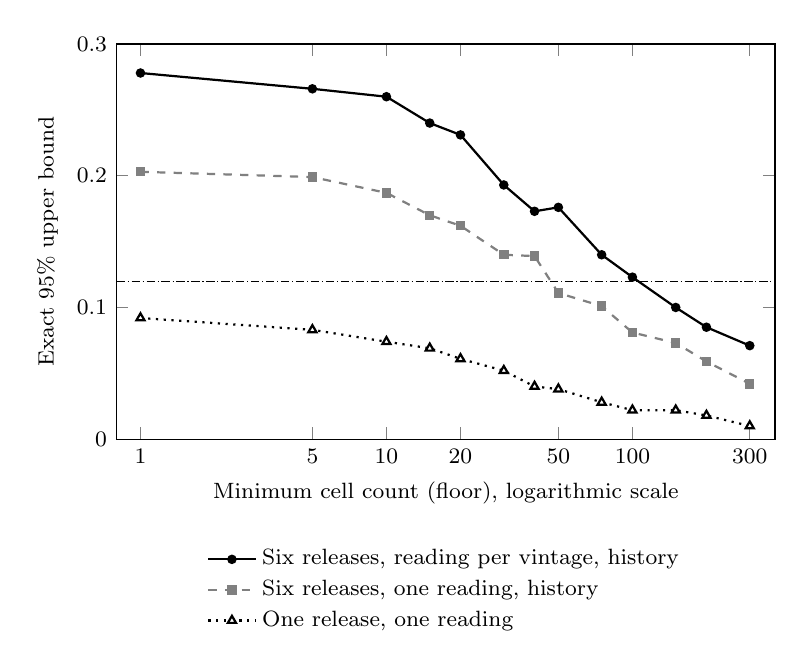
\begin{tikzpicture}
\begin{axis}[width=0.82\textwidth, height=6.6cm,
  xmode=log, xmin=0.8, xmax=380, ymin=0, ymax=0.3,
  xtick={1,5,10,20,50,100,300}, xticklabels={1,5,10,20,50,100,300},
  xlabel={Minimum cell count (floor), logarithmic scale},
  ylabel={Exact 95\% upper bound},
  yticklabel style={/pgf/number format/fixed, /pgf/number format/precision=2},
  label style={font=\footnotesize}, tick label style={font=\footnotesize},
  legend style={font=\footnotesize, at={(0.5,-0.25)}, anchor=north, draw=none},
  legend cell align=left]
\addplot[black, thick, solid, mark=*, mark size=1.3pt] coordinates {
 (1,0.278) (5,0.266) (10,0.260) (15,0.240) (20,0.231) (30,0.193) (40,0.173)
 (50,0.176) (75,0.140) (100,0.123) (150,0.100) (200,0.085) (300,0.071)};
\addlegendentry{Six releases, reading per vintage, history}
\addplot[gray, thick, dashed, mark=square*, mark size=1.3pt, mark options={solid}] coordinates {
 (1,0.203) (5,0.199) (10,0.187) (15,0.170) (20,0.162) (30,0.140) (40,0.139)
 (50,0.111) (75,0.101) (100,0.081) (150,0.073) (200,0.059) (300,0.042)};
\addlegendentry{Six releases, one reading, history}
\addplot[black, thick, dotted, mark=triangle*, mark size=1.7pt, mark options={solid,fill=white}] coordinates {
 (1,0.092) (5,0.083) (10,0.074) (15,0.069) (20,0.061) (30,0.052) (40,0.040)
 (50,0.038) (75,0.028) (100,0.022) (150,0.022) (200,0.018) (300,0.010)};
\addlegendentry{One release, one reading}
\draw[densely dashdotted] (axis cs:0.8,0.12) -- (axis cs:380,0.12);
\end{axis}
\end{tikzpicture}
\caption{Selection draw on the synthetic credit register: the exact one-sided bound at
each floor for three declared adversaries, 4,000 targets per floor, with the tolerance of
0.12 as a dash-dotted line. Adversaries are told apart by line style, shade and marker.
Fixed-sequence selection reads each line from the right and stops at the first point
above the line.}
\label{c05:fig-sequence}
\end{figure}

For the adversary who attacks one release with one reading of a loan's exposure, every
floor passes, the sequence runs to the end, and the chosen floor is 1. For the adversary
who pools the six vintages, holds one reading and knows in which vintages the target's
loan is live, the bounds are 0.042 at 300, 0.059 at 200, 0.073 at 150, 0.081 at 100,
0.101 at 75 and 0.111 at 50, all below 0.12, and 0.139 at 40, which fails. The sequence
stops there and selects 50. For the full pooled adversary, with a reading per live
vintage as well as the history, the sequence passes 300, 200 and 150 and stops at 100,
where the bound is 0.123.
% source: paper/worked_examples.tex, Example ex:selection; artifacts-robustness/robustness.json (selection.pooled_live_history: 100 -> 0.1234)
These selections are the starting points of the floors that the long-form paper
reports for the credit register, before the confirmation step described in the next
section.

\syntheticnote


The full pooled line is not monotone: the bound at 40 is 0.173 and at 50 is 0.176.
% source: artifacts-robustness/robustness.json (selection.pooled_live_history: 40 -> 0.1734, 50 -> 0.1757)
Both lie far above the tolerance, so the disorder does not touch the choice here, but it
shows that monotone bounds cannot be assumed even when the true risks are expected to
fall with the floor. On this register the scan and the fixed sequence chose the same
selection floor for every one of the ten adversaries declared, including the variants
with exposure rounded to one significant figure.
% source: artifacts-robustness/robustness.json (floors[*].smallest_passing == floors[*].fixed_sequence for all ten variants)
That agreement is not the reason to prefer the fixed sequence. The reason is that its
error bound would have held had the two disagreed, and the scan's would not.

\section{The confirmation draw}

The selection step controls the chance of choosing an unsafe floor. It leaves a second
problem in the figure the committee reads. The floor that selection chooses is, by
construction, the last to pass, and so the one whose bound sat closest to the tolerance
among those that passed. Its selection bound is the one most likely to have passed by a
small margin of luck, and a decision record that quotes it quotes the most optimistic
number the procedure produced. The remedy is to audit the chosen floor again on a second
draw of targets, independent of the first, and to carry that confirmation into the
record.

\begin{definition}[Confirmation with fallback]\label{c05:def-confirm}
Let $\hat\theta$ be the setting chosen by fixed-sequence selection. On a second draw of
targets, independent of the selection draw, compute the bound at $\hat\theta$. If it
passes, report $\hat\theta$ with its confirmed bound. If it fails, move to the next more
protective setting in the order and compute its bound on the same second draw, and
continue towards the most protective setting until one passes. If none passes, choose
none.
\end{definition}

\begin{proposition}[Fallback keeps the error bound]\label{c05:prop-confirm}
Under Definitions~\ref{c05:def-fixedseq} and~\ref{c05:def-confirm}, the probability that
the reported setting is unsafe is at most $\alpha$.
\end{proposition}

The reason is that fallback only moves towards protection. Every setting more protective
than $\hat\theta$ also passed the selection sequence, so the reported setting is always
one that passed selection, and the argument of Proposition~\ref{c05:prop-fixedseq} covers
every such setting at once: any unsafe setting can pass selection only if the first unsafe
setting in the order passes, which has probability at most $\alpha$. The guarantee rests
on the selection step alone. The confirmation draw adds a fresh figure for the record and
guards against reporting a floor that passed by chance near the line. What fallback must
never do is move the other way. Choosing a less protective setting after a failed
confirmation, or after seeing that a setting below the first failure would have passed on
the confirmation draw, is a scan with extra steps.

\begin{example}[Confirmation with fallback on the register]\label{c05:ex-confirm}
The adversary who pools six vintages with one reading and the history shows the procedure
at work. Selection chose 50. On the confirmation draw the same attack at 50 named the
target for 458 of 4,000 targets, a rate of 0.115 with a bound of 0.123, above the
tolerance. The procedure moved to the next stricter floor, 75, where 384 of 4,000 targets
were named, a rate of 0.096 with a bound of 0.104, and 75 became the floor.
% source: paper/worked_examples.tex, Example ex:selection (458/4,000, 0.115, 0.123; 384/4,000, 0.096, 0.104)
The full pooled adversary, selected at 150, confirmed there at 0.101 with a bound of
0.109.
% source: paper/generated/table_robustness.tex (150, 0.101 (0.109))
The single-release adversary confirmed at a floor of 1 with 0.084 and a bound of 0.092.
% source: paper/generated/table_robustness.tex (1, 0.084 (0.092))
\end{example}


When Naledi presented these results the chair asked the question that a committee always
asks at this point: if 50 failed by so little, why not 40, which would keep more loans?
The answer was in the record. Forty had failed selection at 0.139, and it was the first
failure in the declared order, so the procedure never reached the question of whether
some later draw might pass it. Falling back to 75 kept the error bound, because 75 had
already passed at selection. Choosing 40 or 30 after seeing these numbers would not have
kept it. The chair accepted the floor of 75 for that adversary.

\section{What the floors cost}

Tomás's question was about the full pooled adversary, because a researcher who receives
six monthly files and can see which loans appear in which month holds exactly that
adversary's information. Its floor was 150. At 150 the release keeps 20 per cent of the
loans of the first vintage, 4 per cent of the exposure and no loan to a large firm; at
75 it keeps 45 per cent of loans and 11 per cent of exposure.
% source: paper/generated/table_robustness.tex (Loans, Exposure columns); paper/bis_ifc_full.tex lines 2264-2268
Large firms carry the largest exposures and sit in the thinnest cells, so they are the
first to go. A file that meets the tolerance against an adversary who knows loan
histories has lost the borrowers that concentration and supervisory research are about.

The insider fares worse. Pieter, a credit analyst at a reporting lender, knows the
exposure of his own institution's loans almost exactly, and the declared insider
adversary reads exposure with an error of 0.01 on the log scale. No floor on the menu
stops it: its success is 0.772 with no suppression and still 0.416 at a floor of 300,
because a precise reading of exposure separates candidates in a cell of any size.
% source: paper/bis_ifc_full.tex lines 2241-2243; paper/generated/table_robustness.tex (insider: none); scripts/programme_robustness.py (INSIDER_SD = 0.01)
A minimum cell count is the wrong lever for that adversary, and the fixed sequence
reports this plainly: its first test, at 300, fails, and it chooses none.

The committee's decision followed. Against an adversary who pools vintages and knows
the histories, a loan-level public or scientific-use file was the wrong product. Tomás
was offered access to the loan-level file in the Bank's secure environment, where the
declared adversary no longer holds the file and the Five Safes treat the access route as
a control of its own \citep{desai2016}, together with aggregates for anything he wished
to publish. The floors behind that decision are synthetic, and a central bank would have
to reproduce them on its own register before relying on their values. The procedure that
produced them does not depend on the register.

\section{Several adversaries, subgroups and tolerances}

A committee usually declares more than one adversary for a release, and it may require
every subgroup of targets, such as every firm size class, to meet the tolerance. Both
requirements fit the fixed sequence without any division of $\alpha$. At each setting the
committee requires every declared attack, or every subgroup, to pass. That is an
intersection--union test (Proposition~\ref{c04:prop-iut}) and is valid at level $\alpha$
as it stands. Ordering the settings and stopping at the first failure then gives a fixed
sequence of intersection--union tests.

\begin{corollary}[A fixed sequence of intersection--union tests]\label{c05:cor-chain}
Let each setting $\theta_\ell$ carry several coordinates, one for each declared attack or
subgroup, each with a bound valid at level $\alpha$, and let $\theta_\ell$ pass when every
coordinate passes. Fixed-sequence selection over $\theta_1, \dots, \theta_L$ chooses a
setting at which some coordinate's true risk exceeds $\tau$ with probability at most
$\alpha$.
\end{corollary}

The long-form paper runs this choice as a release chain with all three outside attacks as
coordinates. Over 20 independent target streams it chose 150 in 19 and 100 once, against
an estimated true floor of 100, and no stream chose an unsafe floor.
% source: paper/bis_ifc_full.tex lines 2305-2311
The gap to 100 comes from the full attack's risk at that floor, 0.116, which lies so
close to the tolerance that an audit of practical size certifies it only by chance.
% source: paper/bis_ifc_full.tex lines 2311-2313; paper/worked_examples.tex Example ex:length
Chapter~6 describes how that chain monitors its evidence as it arrives. The subgroup
control is stricter again: with every size class required to pass, the single-release
floor is 20, pooling with the history needs 200, and for the full attack no floor up to
200 passes.
% source: paper/generated/table_robustness.tex (Subgroup column)
Those subgroup floors were chosen by the same fixed sequence but were not confirmed on a
second draw, and a record that used them should say so.

The tolerance belongs to the declaration as well, and repeating the selection at other
tolerances, from the same draw, shows how much it moves the answer. At a tolerance of 0.05 the
single-release floor is 40, pooling with the history needs 300, and the full attack has
no floor up to 300. At 0.20 the three floors are 1, 5 and 30.
% source: paper/generated/table_tolerance_floors.tex
Across that range the floor moves by an order of magnitude. A committee that is unsure
of its tolerance should read the whole table before the selection draw is run, and
should fix the tolerance before it is. A tolerance chosen after the floors are known is a
scan over tolerances, and it inflates the error in the same way as a scan over settings.

\section{Menus that are not a line}

The credit register's menu was one lever, and its order was obvious. The household
grid of the long-form paper had three levers, band width, occupation groups and minimum
cell count, and 45 settings that no single ordering of protection ranks without
judgement. Proposition~\ref{c05:prop-fixedseq} allows any order fixed independently of
the selection draw, and that permission is what makes a multi-lever grid workable. An
analyst can run a pilot draw, estimate the frontier from it, and declare the path through
the grid that the pilot suggests, from the most protective nondominated setting towards
the least. The selection draw and the confirmation draw are then run fresh on that path.
The pilot may be as informal as the analyst likes, because nothing it produces is used as
evidence. The settings off the path are not tested, and the record should list them so
that a reviewer can see what was left out. Chapter~14 uses the same division of labour
when a model proposes the order and an independent audit decides.

\section{A choice that keeps its error}

The question of this chapter was how a committee can choose a protection setting from a
menu, using the same simulated evidence that certifies it, and keep the chance of
releasing an unsafe setting at its stated level. The answer is to fix the order of the
menu, from the most protective setting down, before any attack is run; to test the
settings in that order with the level-$\alpha$ bound and stop at the first that fails; to
choose the last setting that passed; and to confirm that setting on an independent draw,
moving only towards more protection if confirmation fails. The chance of choosing an
unsafe setting is then at most $\alpha$ whatever the true risks, and the figure in the
record comes from a draw that did not choose it. Scanning the grid for the least costly
setting that passes gives up that control in proportion to the number of unsafe settings
near the line, which a committee cannot know in advance. The fixed sequence costs utility
only when the bounds are out of order past the first failure, and on the credit register
it cost nothing. It does not change what the menu can achieve: when no setting on it
meets the tolerance, as for the insider, the sequence says so at its first step, and the
answer is a different product.

\begin{inpractice}\sloppy
Before running any attack, write into the decision record the menu of settings, its order
from most to least protective, the tolerance, the error level, the declared adversaries
and subgroups, and the number of targets in each draw. Run the selection draw down the
order and stop at the first failure. Run the confirmation on a fresh draw at the chosen
setting, and if it fails, move only to more protective settings. Report the confirmed
figure with its bound, and state any floor that was selected but not confirmed. Do not
present, in any table the committee reads, results for settings below the first failure.

\smallskip\noindent\textit{In the software.} The selection used for the credit register
is the function \texttt{fixed\_sequence} in \texttt{scripts/programme\_robustness.py},
which also computes the scan's choice (\texttt{smallest\_passing}) for comparison and runs
the confirmation draw; \texttt{scripts/robustness\_table.py} applies the fallback of
Definition~\ref{c05:def-confirm} in \texttt{confirmed\_floor}. The release chain of
Corollary~\ref{c05:cor-chain} is \texttt{privacy\_risk.adaptive\_audit.ReleaseChain},
which refuses to open a setting before the previous one has passed. The household grid
and its frontier are produced by \texttt{privacy\_risk.experiments.mechanism\_grid}. The
selection rule is short:
\begin{lstlisting}
def fixed_sequence(levels: list[int], passed: dict) -> int | None:
    """Test from the strictest level down and stop at the first failure."""
    chosen = None
    for k in sorted(levels, reverse=True):
        if not passed[k]:
            break
        chosen = k
    return chosen
\end{lstlisting}
For a minimum cell count a larger value is more protective, so sorting in reverse puts
the strictest floor first.
\end{inpractice}

\section{Proofs}

\begin{proof}[Proof of Proposition~\ref{c05:prop-exist}]
Let $g(\theta) = \sup_{t\in T}\overline{R}_{1-\alpha}(t,\theta)$ and
$\Theta_\tau = \{\theta \in \Theta : g(\theta) \le \tau\}$. Lower semicontinuity of $g$
means that every sublevel set of $g$ is closed, so $\Theta_\tau$ is closed. A closed
subset of a compact space is compact, and $\Theta_\tau$ is non-empty by assumption. Let
$u^\ast = \sup_{\Theta_\tau}U$ and take $\theta_n \in \Theta_\tau$ with
$U(\theta_n) \to u^\ast$. By compactness a subsequence converges to some
$\theta^\ast \in \Theta_\tau$, and upper semicontinuity gives
$U(\theta^\ast) \ge \limsup U(\theta_n) = u^\ast$. Hence $u^\ast$ is finite and attained
at $\theta^\ast$, which solves \eqref{c05:eq-opt}.
\end{proof}

\begin{proof}[Proof of Proposition~\ref{c05:prop-scan}]
The scan chooses a setting only if that setting passes, so it chooses an unsafe setting
only if some $\theta \in H$ passes. By Boole's inequality,
$\Prob\{\text{some } \theta \in H \text{ passes}\} \le \sum_{\theta\in H}\Prob\{\theta
\text{ passes}\} \le |H|\alpha$, and every probability is at most one.

Now suppose every unsafe setting is less protective than every safe one. If some unsafe
setting passes, the least protective passing setting is either that setting or another
setting still less protective, and every setting less protective than an unsafe one is
unsafe, since all safe settings are more protective than all unsafe ones. So the scan
chooses an unsafe setting. Conversely, if no unsafe setting passes, the scan chooses a
safe setting or none. The scan therefore chooses an unsafe setting exactly when some
unsafe setting passes. With independent draws the pass events are independent, so the
probability that none of the unsafe settings passes is $\prod_{\theta\in H}(1-p_\theta)$,
and its complement is \eqref{c05:eq-scan}.
\end{proof}

\begin{proof}[Proof of Proposition~\ref{c05:prop-fixedseq}]
Condition on the order, which is independent of the selection draw, so that each bound
keeps its level-$\alpha$ property given the order. If no setting is unsafe there is
nothing to prove. Otherwise let $i^\ast$ be the smallest index with $\theta_{i^\ast}$
unsafe. The procedure chooses $\theta_j$ only if $\theta_1, \dots, \theta_j$ all pass,
so the set of settings that the procedure passes is an initial segment of the order. The
procedure chooses an unsafe setting $\theta_j$ only if $j \ge i^\ast$, and then
$\theta_{i^\ast}$ lies in the initial segment and passed. Hence
\[
\Prob\{\text{an unsafe setting is chosen}\} \le
\Prob\{\theta_{i^\ast}\text{ passes}\} \le \alpha,
\]
the last step because $\theta_{i^\ast}$ is a fixed unsafe setting given the order and its
bound is valid at level $\alpha$. Integrating over the order preserves the bound. The
argument uses only the identity of the first unsafe setting, not the order of the true
risks \citep{maurer1995}.
\end{proof}

\begin{proof}[Proof of Proposition~\ref{c05:prop-compare}]
Fix a realisation of the selection draw. If $\theta_1$ fails, fixed-sequence selection
chooses none; the scan chooses the least protective passing setting if there is one, and
`none' counts as the most protective outcome, so the claim holds. Otherwise let
$\theta_m$ be the fixed-sequence choice, so that $\theta_1,\dots,\theta_m$ pass and
$\theta_{m+1}$, if it exists, fails. The scan's choice is the passing setting with the
largest index, which is at least $m$ because $\theta_m$ passes. So the scan's choice is
at least as far down the order, that is, no more protective. The two coincide if and only
if no $\theta_j$ with $j > m+1$ passes, which is the condition stated. If utility
increases strictly along the order, the solution of \eqref{c05:eq-opt} over the grid with
the realised bounds is the passing setting with the largest index, which is the scan's
choice, and under the stated condition it equals the fixed-sequence choice.
\end{proof}

\begin{proof}[Proof of Proposition~\ref{c05:prop-confirm}]
The reported setting is $\hat\theta$ or a setting earlier in the order than
$\hat\theta$. By Definition~\ref{c05:def-fixedseq}, every setting from $\theta_1$ to
$\hat\theta$ passed the selection draw. Hence the reported setting passed the selection
draw. If it is unsafe, some unsafe setting passed the selection draw; as in the proof of
Proposition~\ref{c05:prop-fixedseq}, the settings that pass form an initial segment, so
the first unsafe setting $\theta_{i^\ast}$ passed. That event has probability at most
$\alpha$. The confirmation draw enters only through which of the passed settings is
reported, and every passed setting is covered by the same event, so its outcome does not
affect the bound.
\end{proof}

\begin{proof}[Proof of Corollary~\ref{c05:cor-chain}]
Call $\theta_\ell$ unsafe if some coordinate has true risk above $\tau$. Let
$\theta_{i^\ast}$ be the first unsafe setting in the order. By
Proposition~\ref{c04:prop-iut}, applied to the coordinates of $\theta_{i^\ast}$, the
probability that $\theta_{i^\ast}$ passes is at most $\alpha$. The rest of the proof of
Proposition~\ref{c05:prop-fixedseq} applies without change, since it used only the
level-$\alpha$ property of the first unsafe setting's pass event.
\end{proof}
